\documentclass{article}
\usepackage{tikz}
\begin{document}

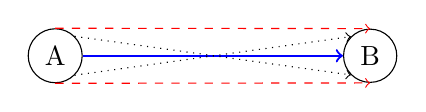
\begin{tikzpicture}[scale=1]

  % --- Define nodes ---
  \node[draw, circle] (A) at (0,0) {A};
  \node[draw, circle] (B) at (4,0) {B};

  % --- Connect using anchors ---
  % From east side of A to west side of B
  \draw[->, thick, blue] (A.east) -- (B.west);

  % From north of A to north of B
  \draw[->, red, dashed] (A.north) -- (B.north);

  % From south of A to south of B
  \draw[->, red, dashed] (A.south) -- (B.south);

  % --- Corner anchors ---
  % From north east of A to south west of B
  \draw[->, dotted, black] (A.north east) -- (B.south west);

  % From south east of A to south west of B
  \draw[->, dotted, black] (A.south east) -- (B.north west);

\end{tikzpicture}

\end{document}
